% =====================================================================================================
%
%  INTRODUCTION
%
% =====================================================================================================
\begingroup
\renewcommand{\cleardoublepage}{}
\renewcommand{\clearpage}{}
\chapter*{Introduction}\label{chap:introduction}
\addcontentsline{toc}{chapter}{Introduction}
\renewcommand{\chapter}[2]{}%q

\lettrineabstract{We present a highly parameter-efficient approach for Question Answering (QA) that significantly reduces the need for extended BERT fine-tuning. Our method uses information from the hidden state activations of each BERT transformer layer, which is discarded during typical BERT inference. Our best model achieves maximal BERT performance at a fraction of the training time and GPU/TPU expense. Performance is further improved by ensembling our model with BERT’s predictions. Furthermore, we find that near optimal performance can be achieved for QA span annotation using less training data. Our experiments show that this approach works well not only for span annotation, but also for classification, suggesting that it may be extensible to a wider range of tasks.}\footnote{\textit{BERTVision} - so named for our method of peering within BERT for the signal hidden therein.}
\footnote{See GitHub repository: \href{https://github.com/cbenge509/BERTVision}{BERTVision}}

\begin{figure*}[!h]
	\floatbox[{\capbeside\thisfloatsetup{capbesideposition={right,top},capbesidewidth=8cm}}]{figure}[\FBwidth]
	{\caption{Architecture of our best model in relation to BERT. \textbf{Left}: BERT and its span annotation inference process. \textbf{Right}: For our model, BERT embeddings are first transformed through our custom adapter layer. Next, the last two dimensions are flattened. Optionally, a skip connection is added between the sequence outputs of the final BERT layer and this flattened representation. This is present in the best model discovered at 3/10 of an epoch, but was not necessary for the best model discovered at 1 full epoch. This tensor is then projected down to (386, 2) with a densely connected layer and split on the last axis into two model heads.  These represent the logits of the start-span and end-span position.}\label{fig:architecture}}
	{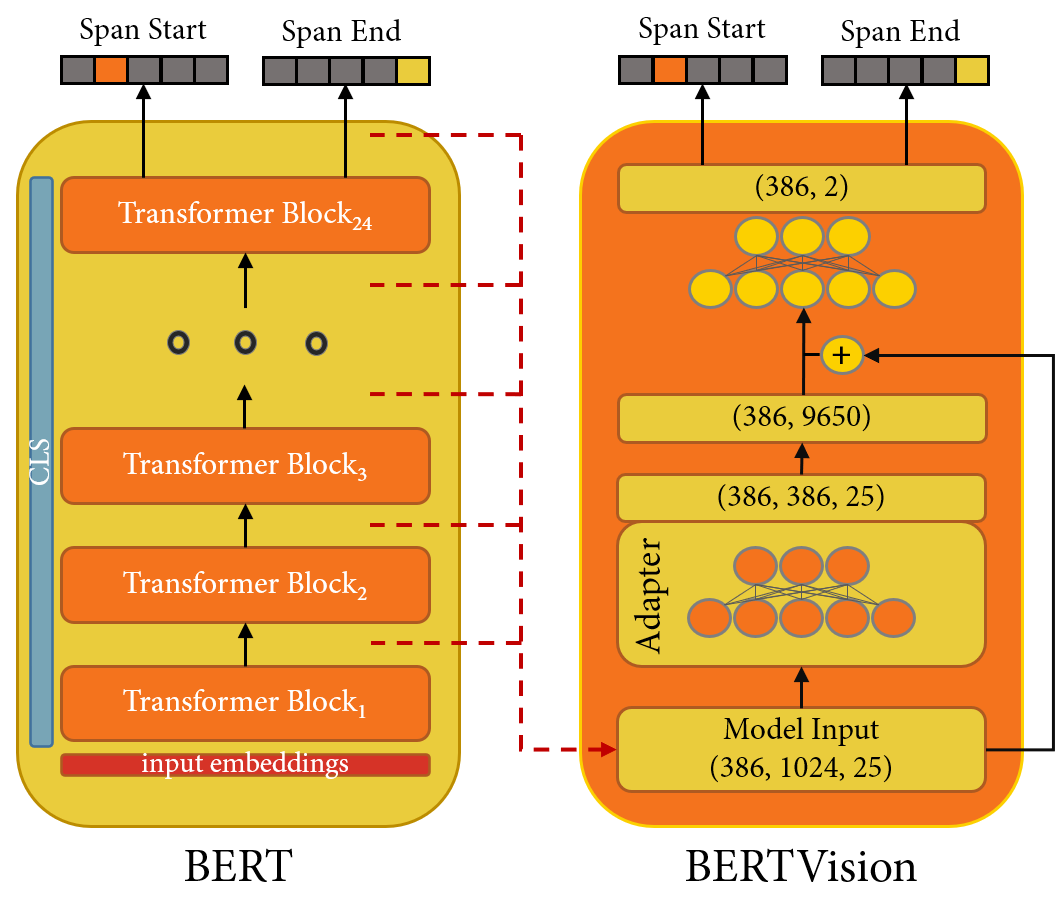
\includegraphics[width=7.5cm]{images/BERTVision_QA_Model.png}}
\end{figure*}

%----------------------------------------------------------------------------------------
%	ARTICLE CONTENTS
%----------------------------------------------------------------------------------------
\fakesection{Introduction}
\label{sec:Introduction}

\doubleline

The introduction of Transformers \cite{Vaswani2017} has significantly advanced the state-of-the-art for many NLP tasks. The most well-known Transformer-based model is BERT \cite{Devlin2019}. The standard way to use BERT on a specific task is to first download pre-trained weights for the model, then fine-tune these weights on a supervised dataset. However, this procedure can be quite slow, and at times prohibitive for those without a powerful GPU/TPU, or those with limited CPU capacity. Smaller Transformers, such as DistilBERT \cite{sanh2019distilbert}, can fine-tune up to 60\% faster. However, such models tend to consistently underperform full-size BERT on a wide range of tasks. A method that reduces fine-tuning but maintains the same or better performance would make BERT more accessible for practical applications.

To develop our method, we drew inspiration from previous works that use BERT for feature extraction rather than for fine-tuning \citep{Zhu2020IncorporatingBI, Chen_2020}. For example, Zhu et al. showed that the sequence outputs from the final BERT layer can be used as contextualized embeddings to supplement the self-attention mechanism in an encoder/decoder neural translation model. This led to an improvement over the standard Transformer model in all tested language pairs on standard metrics (BLEU score \cite{Papineni02bleu:a}).

One characteristic these studies share with typical BERT inference is that only information from the final layer of BERT is used. However, a study by \cite{tenney-etal-2019-bert} suggests that all layers of BERT carry unique information. By training a series of classifiers within the edge probing framework \cite{DBLP:journals/corr/abs-1905-06316}, the authors computed how much each layer changes performance on eight labeling tasks, and the expected layer at which the model predicts the correct labels. The discovery is that syntactic information is encoded earlier in the network, while higher level semantic information comes later. Furthermore, classifier performance generally increases for all tasks when more layers are accounted for, starting from layer 0, suggesting that useful information is being incorporated at each progressive layer. Others, such as \cite{van_Aken_2019}, looked specifically at QA with SQuAD and published similar findings. Their work suggests that different layers encode different information important for QA.

\cite{ma2019universal} showed that a simple averaging of only the first and last layers of BERT results in contextualized embeddings that performed better than only using the final layer. The authors evaluated this approach on a variety of tasks such as text classification and question-answering. Together, these works suggest that the hidden state activations within BERT may contain unique information that can be used to augment the final layer. That said, the exact way of doing this requires further exploration.

In this work, we leverage the findings by Tenney and Ma as inspiration for developing a solution with a two-fold goal: $1.$ Reduce expensive BERT fine-tuning; $2.$ Maintain or exceed BERT-level performance in the process. To do so, we extract the information-rich hidden states from each encoder layer and use the full embeddings as training data. We demonstrate that, for two question-answering tasks, even our simple architectures can match BERT performance at a fraction of the fine-tuning cost. Our best model saves on one full epoch of fine-tuning, and performs better than BERT, suggesting that our approach may be a desirable substitute to fine-tuning until convergence.

%----------------------------------------------------------------------------------------
\endgroup